\documentclass[sigconf]{acmart}

\usepackage{graphicx}
\usepackage{hyperref}
\usepackage{todonotes}

\usepackage{endfloat}
\renewcommand{\efloatseparator}{\mbox{}} % no new page between figures

\usepackage{booktabs} % For formal tables

\settopmatter{printacmref=false} % Removes citation information below abstract
\renewcommand\footnotetextcopyrightpermission[1]{} % removes footnote with conference information in first column
\pagestyle{plain} % removes running headers

\newcommand{\TODO}[1]{\todo[inline]{#1}}

\usepackage{listings}
\usepackage{color}
% \usepackage[parfill]{parskip}

\definecolor{dkgreen}{rgb}{0,0.6,0}
\definecolor{gray}{rgb}{0.5,0.5,0.5}
\definecolor{mauve}{rgb}{0.58,0,0.82}

\lstset{frame=tb,
  language=Python,
  aboveskip=3mm,
  belowskip=3mm,
  showstringspaces=false,
  columns=flexible,
  basicstyle={\small\ttfamily},
  numbers=none,
  numberstyle=\tiny\color{gray},
  keywordstyle=\color{blue},
  commentstyle=\color{dkgreen},
  stringstyle=\color{mauve},
  breaklines=true,
  breakatwhitespace=true
  tabsize=3
}

\def\bZ{\mathbb{Z}}
\def\bN{\mathbb{N}}
\def\bR{\mathbb{R}}
\def\bC{\mathbb{C}}
\def\bQ{\mathbb{Q}}

\begin{document}
\title{Comparison between different classification algorithms in Digit Recognizer}


\author{Junjie Lu}
% \orcid{1234-5678-9012}
\affiliation{
  \institution{Indiana University Bloomington}
  \city{Bloomington} 
  \state{Indiana} 
  \postcode{47408}
}
\email{junjlu@iu.edu}


\author{Yuchen Liu}
\affiliation{
  \institution{Indiana University Bloomington}
  \streetaddress{1750 N Range Rd}  
  \city{Bloomington} 
  \state{Indiana} 
  \postcode{47408}
}
\email{liu477@iu.edu}

\author{Wenxuan Han}
\affiliation{
  \institution{Indiana University Bloomington}
  \streetaddress{1150 S Clarizz Blvd}
  \city{Bloomington}
  \state{Indiana}
  \postcode{47401-4294}
}
\email{wenxhan@iu.edu}


% The default list of authors is too long for headers}
% \renewcommand{\shortauthors}{G. v. Laszewski}
\makeatletter
\def\subsubsection{\@startsection{subsubsection}{3}%
  \z@{.5\linespacing\@plus.7\linespacing}{.1\linespacing}%
  {\normalfont\itshape}}
\makeatother

\begin{abstract}

Digit Recognizer is becoming more and more important in many different areas, such as zip code recognizer, banking receipt and balance sheet. Many technology companies are trying to use Big Data to develop more efficient and accurate algorithm for Digit Recognizer. This project uses Digit Recognizer data set from Kaggle.com. There are more than 42000 samples in the data set. Each sample contains 784 features which contain pixel information from a $28*28$ graph. Each pixel has a value between 0 to 255. We use binary classification technique for data cleaning and PCA for feature extraction. For the classification model, we choose five most commonly used classification algorithms, which include Decision Tree (DT), Naive Bayes (NB), Logistic Regression (LR), Random Forest (RF) and Support Vector Machine (SVM). From the result, SVM classifier on PCA data produces the highest accuracy with 0.9813. The time spend is 127 seconds. Naive Bayes classifier on PCA data spends the least amount of time to finish the classification task. It takes less one second and reaches a 0.8651 accuracy.

\end{abstract}

\keywords{I523, HID213, HID214, HID209, Big Data, Digit Recognition, Cross Validation,  Decision Tree, Naive Bayes, Logistic Regression, Random Forest, Support Vector Machine}


\maketitle



\section{Introduction}

People have made a great improvement in digital recognition in recent years. And it plays significant roles in many different areas. Zip code recognizer can scan zip code for post office automatically. Recognizer in banks can help managing user account by scanning their account number. They help people a lot in increasing working efficiency. And many new productions use digital recognition to authenticate password. In this situation, the accuracy and efficiency of recognition become more and more essential and methods in order to increase the accuracy and efficiency are also required.

Fortunately, people have already developed many different types of techniques to avoid faults and decrease running time in recent few years. Several algorithms will be mentioned here. Logistic regression, the most frequently used algorithm in the field of machine learning, also has a good performance in digital recognition. Decision tree is commonly used in decision analysis. It can identify strategies to get a result, in this case, it can also play an important role in digital recognition. Naive Bayes classifier would also be used. Random forest is also a widely used technique in the field of classification and regression. Its special structure with the multitude of decision trees would help it get a fantastic result. Support vector machine can efficiently perform non-linear classification hence it also be considered frequently. These algorithms have different structures so that they have different performance. We can also observe running time and accuracy of different algorithms with different kind of data. In this paper, we are going to talk about this and make the comparison between algorithms in accuracy and efficiency.

\section{Experiment Preparation}

In this paper, we choose the data of Digit Recognizer from Kaggle.com in order to test different classification algorithms \cite{kaggle}. The goal of this experiment is to correctly identify digits from a data set of tens of thousands of handwritten images. Thus, we could compare the pros and cons of each technique through the recognition accuracy and time-consuming.

\subsection{Data Set Description}

In train.csv data file, it contains $42000$ gray-scale images of hand-drawn digits, from zero through nine. Each image is a $28 \times 28$ pixels matrix with a total of 784 pixels \cite{kaggle}. Each pixel has a single pixel-value which is an integer from 0 to 255 associated with it, indicating the lightness or darkness of that pixel (higher numbers meaning lighter). In this experiment, we have plotted the graph in order to see the appearance of these digits easily. Figure 1 shows the first 70 samples.
\begin{figure}[!ht]
\centering
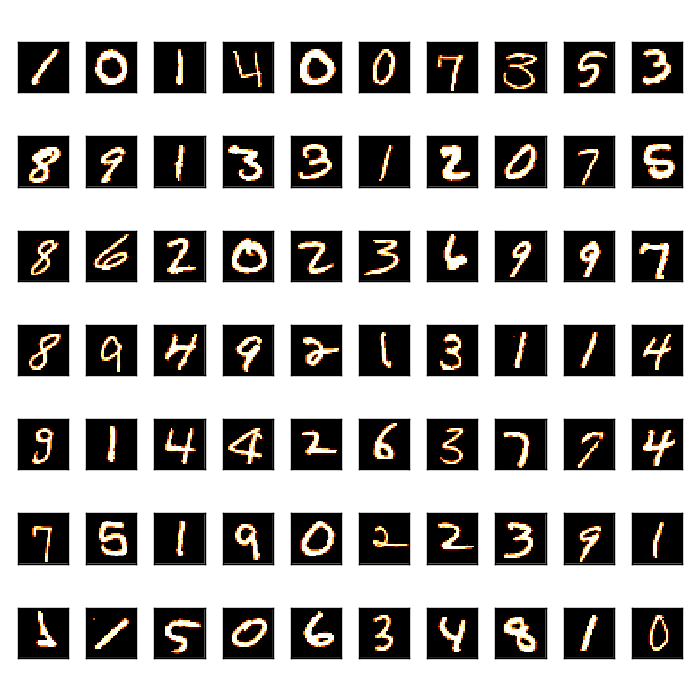
\includegraphics[]{images/data_samples}
\caption{70 samples of hand-drawn digits in this data set.}
\end{figure}

The training data set has 785 columns. The first column called ``label'', is the digit that was drawn by the user. The rest of the columns contain the pixel-values of the associated image. Each pixel column in the training set has a name like $pixelx$, where $x$ is an integer between 0 and 783. To locate a pixel on the image, suppose that we have decomposed $x$ as $x=i*28+j$, where $i$ and $j$ are integers between 0 and 27. Then $pixelx$ is located in row $i$ and column $j$ of this matrix \cite{kaggle}. Visually, if we omit the ``pixel'' prefix, the pixels make up the image like the following form:
$$
  \begin{matrix}
   000 & 001 & 002 & 003 & \cdots & 026 & 027 \\
   028 & 029 & 030 & 031 & \cdots & 054 & 055 \\
   056 & 057 & 058 & 059 & \cdots & 082 & 083 \\
   \vdots & \vdots & \vdots & \vdots & \vdots & \vdots & \vdots \\
   728 & 729 & 730 & 731 & \cdots & 754 & 755 \\
   756 & 757 & 758 & 759 & \cdots & 782 & 783
  \end{matrix}
$$

\subsection{Data Cleaning}

As we mentioned above, it can be seen from both the figure and the pixel-value that the value varies from 0 to 255, which means each feature is a continuous value. Thus, it is possible that such continuous values might affect our later feature selection. Our observation shows that the values are not very high at the boundaries of 0 and $>0$. So here exist three ways to handle it \cite{data_clean}:
\begin{enumerate}
    \item Not do any processing on image;
    \item Binarize the image. That is, for the values which are 0, keep them as 0; for the values which are greater than 0, change to 1;
    \item Binarize the image by setting a threshold. That is, for the values which are greater than this threshold, change to 1; otherwise, change to 0.
\end{enumerate}

Obviously, method (2) and (3) will cause the loss of the original information. However, this information may not as important as our expected during the execution of classification algorithms, it could play a positive role in increasing the performance without reducing the accuracy.

In our experiment, we selected method (2) to clean the raw data. The following part of codes shows this operation.
\begin{lstlisting}
from numpy import *

# The data is from 0-255 for each cell.
# Normalize data by set all value > 0 to 1
def data_clean(data):
    m, n = shape(data)
    new_data = zeros((m, n))
    for i in range(m):
        for j in range(n):
            if data[i, j] > 0:
                new_data[i, j] = 1
            else:
                new_data[i, j] = 0
                
    print("Data clean completed.")
    return new_data
\end{lstlisting}

\subsection{Feature Extraction}

Dimension reduction in the field of machine learning refers to using a mapping method to map the data points in the original high-dimensional space into the low-dimensional space. The essence of dimension reduction is to learn a mapping function \(f:x->y\), where x is the expression of the original data point, y is the low-dimensional vector representation after the data point mapping \cite{feature_extra}. 

The reason why we use data after dimension reduction is that the redundant information and noise information are contained in the original high-dimensional space, which reduces the accuracy of our model. By dimension reduction, we hope to reduce the error caused by redundant information and improve the accuracy of identification. We also hope to find the intrinsic structure of the data structure through the dimension reduction algorithm. Also, in this example, there are 784 features in our data. Space, time and computation complexity are all unacceptable. There are many different dimension reduction algorithms for us to choose. In this project, we choose to use Principle Component Analysis (PCA).

\subsubsection{PCA}

Principal Component Analysis (PCA) is the most commonly used method of supervised linear dimension reduction. Its goal is to map high-dimensional data to a low-dimensional representation of space by some kind of linear projection. The variance of the data is expected to be maximized in the projected dimension. By keep the variance of data as high as possible, PCA can reduce the dimension of data and keep the loss of information of the data as a minimum \cite{PCA}.

A common understanding is that if all the points are mapped together, almost all information (such as the distance between points) is lost. If the post-mapping variance is as large as possible, the data points are spread apart to preserve more information. It can be proved that PCA is a linear dimension reduction method that loses the original least data information.

One of the questions we faced while we are using PCA is that: how many components should we choose for the model after dimension reduction. In order to solve this problem, we use Explained Variance as our threshold standard. Explained Variance is an important indicator of PCA dimension reduction. The Explained Variance shows the amount of variance explained by each of the selected components. The first column of the PCA model always explains the most variance and the variance explained will keep decrease as the number of column increase. Generally, a dimension with a cumulative contribution rate of about 90\% is selected as a reference dimension for PCA dimensionality reduction. In this project, in order to get a more accurate result, we choose 95\% as our threshold.

\begin{lstlisting}
from sklearn.decomposition import PCA

def feature_selection(data):
    pca = PCA()
    pca.fit(data)
    ev = pca.explained_variance_
    ev_ratio = []
    for i in range(len(ev)):
        ev_ratio.append(ev[i] / ev[0])

    # select number of component which have a higher ratio
    # than 0.05 with the first components
    n = 0
    for i in range(len(ev_ratio)):
        if ev_ratio[i] < 0.05:
            n = i
            break

    # Then, PCA the model by the number of components
    pca = PCA(n_components=n, whiten=True)
    return pca.fit_transform(data)
\end{lstlisting}

After calculating the explained variance for each component, we decide to choose 30 components for our model. Which shows that there will be 30 features in our model.

\section{Experiment Algorithms}

We aim to select five most commonly used classification algorithms which include Decision Tree, Naive Bayes (NB), Logistic Regression (LR), Random Forest (RF) and Support Vector Machine (SVM). This section offers a broad overview of these algorithms before applying them to the digit recognizer problem to compare their characteristics. Then, the result of the different algorithm on different data will show on a table.

For each algorithm, we use:
\begin{enumerate}
    \item PCA data - data after using PCA to reduce the dimension on raw data
    \item Clean data - data after our data cleaning process, which set all values greater than 0 to 1 in our data
    \item PCA Clean daata - data after using PCA to reduce the dimension on clean data after data cleaning process
\end{enumerate}

\subsection{Cross-Validation}

When we build the model, it is normal to follow the principle of simplification since the simpler model we built, the better performance we will get. However, for some complicated problems, our model will also become more complex which might cause the over-fitting problem. In order to solve this problem, we introduce the cross-validation technique. Cross-validation is a technique to evaluate predictive models by partitioning the original sample into a training set to train the model, and a test set to evaluate it \cite{10f.cv}.

The purpose of cross-validation is to select the model with the optimal parameters. After the model is set up, tuning the parameters is a very time-consuming process. Through cross-validation, we can get the model with the optimal parameters much easier. Here are some steps about cross-validation procedure:
\begin{enumerate}
    \item Prepare the candidate models, $M_1,M_2,M_3,\cdots$ (the model framework is consistent, only different on the parameters);
    \item For each model, use cross-validation to return the accuracy and error rate information of the model, the result should be the average of cross-validation;
    \item Select the best model by comparing the accuracy or error of the different models.
\end{enumerate}

There are some types of cross-validation which are common to use: K-fold cross-validation and Leave-one-out cross-validation.
\begin{itemize}
    \item K-fold: \\
    This method is to divide the data set into $k$ subsets. Each time, select one of the $k$ subsets as the test set and the other $k-1$ subsets become a training set. Then the average accuracy or error across all $k$ trials is computed \cite{10f.cv}. In general, we choose 10 as the value of $k$. 
    \item Leave-one-out (LOO): \\
    This method is K-fold cross-validation taken to its logical extreme, with $k=n$ ($n>k$), the number of data points in the set \cite{10f.cv}. That is, it randomly select $n$ samples as a training set and the rest as a test set. Since the time complexity of this cross-validation is factorial, it is not an appropriate method for big data set.
\end{itemize}

In this project, we use K-fold cross validation technique to reduce over-fitting of our model and increase the accuracy in each model. We use the function $cross\_val\_score$ from the sklearn package. It have several important parameters to set \cite{sklearn.cv}.

\begin{enumerate}
    \item CV: int, cross-validation generator or an iterable, optional
    This parameter determines the cross-validation splitting strategy, which determined the number of fold we need to use. In our project, we use the default 3-fold cross-validation. Because 3-fold provide us the result in a reasonable time and accuracy.
    \item Scoring: string, callable or None, optional, default: None
    The scoring parameter determines what to return after we call the function. We just this parameter to `accuracy', which will return the accuracy between 0 to 1 for each model.
\end{enumerate}

After we receive the result for each validation, we generate the mean of each result and use the result as the accuracy of the model.

\begin{lstlisting}
from datetime import datetime
from sklearn.cross_validation import cross_val_score

def model_acc(data, label, model):
    start = datetime.now()
    acc = cross_val_score(model, data, label, cv=5, scoring="accuracy").mean()
    end = datetime.now()
    time_use = (end - start).seconds
    
    print("Time use: ", time_use)
    print("Accuracy by cross validation: ", acc)
\end{lstlisting}

\subsection{Decision Tree}

\subsubsection{Introduction}

Decision tree builds classification or regression models in the form of a tree structure (either binary or non-binary) \cite{ss.dt}. Each of its non-leaf nodes represents a test on the characteristic attributes, and each leaf node stores a category. The process of decision making using decision tree has the following steps \cite{intro.dm}:
\begin{enumerate}
    \item Start at the root node;
    \item Test the corresponding characteristic attribute of the items that need to be classified;
    \item Select the branch based on the value until the leaf node is reached;
    \item The category of stored in the leaf node is the result.
\end{enumerate}

The decision tree construction process rely on attribute selection metrics in order to choose the attribute which has the capability to divide tuples into different classes best. The key step in constructing a decision tree is split attributes which means to construct different branches according to the different partition of a certain characteristic attribute at a node. The goal of this step is to make each split subset as ``pure'' as possible. Split attributes are divided into three different situations:
\begin{enumerate}
    \item Attributes are discrete values and do not require to generate a binary decision tree. This time, each partition of an attribute becomes a branch;
    \item Attributes are discrete values and require to generate a binary decision tree. This time, a subset of attribute partitions is used for testing, broken down two branches according to ``subordinate to this subset'' and ``not subordinate to this subset'';
    \item Attributes are continuous values. This time, determine a value as a $split\_point$ and generate two branches according to $>split\_point$ and $\leq split\_point$.
\end{enumerate}

There are many attribute selection metric algorithms (e.g. ID3, C4.5, CART, etc.), generally using top-down recursive method with non-backtrack greedy strategy. In our experiment, we applied optimized version of the Classification And Regression Trees (CART) algorithm from scikit-learn library.

The CART algorithm uses a binary recursive segmentation technique \cite{cart}: the current sample set is divided into two sub-sample sets, so that each non-leaf node have two branches. Therefore, the decision tree generated by the CART algorithm is a concise binary tree with the root node represents a single input variable ($x$) and a split point on that variable and the leaf nodes contain an output variable ($y$) which has the capability to make a prediction \cite{cart}.

The first key step of CART algorithm is creating the tree model, it examines each variable and all possible partitions of this variable to observe the best partitions. For discrete values such as $U=\{x, y, x\}$, there are three cases of partitions \cite{sklearn.dt}:
\[
    \{\{x,y\},\{z\}\},\{\{x,z\},\{y\}\}, \{\{y,z\},\{x\}\}
\]
except $\varnothing$ and $U$; for continuous values, it introduces the idea of ``split point''. Suppose one attribute of a sample has $n$ continuous values, it then has $n-1$ splitting points where each of them is the average of two consecutive values $(a[i]+a[i+1])/2$. Partitions of each attribute are sorted by the amount of impurities that they can reduce. The reduction of impurities could use the most popular method of impurity metric which is: Gini index. If we use $k$ ($k= 1,2,3,\cdots, C$) to represent the class, where $C$ is the dependent variable number of the category set. Thus, the Gini impurity of a Node $A$ could be defined as \cite{sklearn.dt}:
\[
    Gini(A)=1-\sum_{k=1}^{C} p_{k}^2
\]

Where $p_{k}$ denotes the probability of observation points which belong to class $k$. When $Gini(A)=0$, all samples belong to the same class. When $Gini(A)$ is the maximum, which is $\dfrac{(C-1)C}{2}$, all classes occur with the same probability in nodes.

The second key idea in the CART process is to prune the trees of the training set with independent validation data sets. Analyzing the recursive tree construction of classification and regression tree, it is easy to find that there exists a data over-fitting problem \cite{cart}. In the construction of decision tree, many branches reflect the abnormality in training data due to the noises or outliers inside. Using such decision tree to classify the data with unknown categories, the accuracy of classification is not high. So it is essential to detect and subtract these branches. Generally, tree pruning method uses statistical metrics, subtract the least reliable branches, which results in faster classification and improves the ability to separate correctly from the training data. The CART algorithm often adopts the post-pruning method, which is implemented by pruning the branches in a fully grown tree. By deleting the branch of the node to cut tree nodes, the bottom non-pruned node becomes a leaf.

The following part of codes shows how we called CART algorithm in our experiment.
\begin{lstlisting}
# Import Library
from sklearn import tree

def dt_classifier(data, label, data_type):
    dt_model = tree.DecisionTreeRegressor()
    dt_model.fit(data, label)
    print("Test " + data_type + " using DT: ")
    
    # Train the model using the training sets and check score
    model_acc(data, label, dt_model)
\end{lstlisting}

\subsubsection{Advantage and Disadvantage}

Decision Tree has advantages as follow \cite{DT}:
\begin{enumerate}
    \item Decision trees are easy to understand and implement, and people have the ability to understand what the decision tree means by explaining it.
    \item Data preparation is often simple or unnecessary for decision trees, and other techniques often require first generalizing data, such as removing redundant or blank attributes.
    \item Feasible and effective results for large data sources in a relatively short period of time.
    \item Not sensitive to missing values
    \item Can handle irrelevant feature data
    \item High efficiency. Decision tree only needs to build once. The maximum number of calculations for each prediction does not exceed the depth of the decision tree
\end{enumerate}

Decision Tree also has disadvantages as follow \cite{DT}:
\begin{enumerate}
    \item Hard to predict features with continues value
    \item Need to do a lot of data reprocessing work for time-series data
    \item When the category is too large, the error rate may increase.
    \item It does not look good when dealing with data that has a strong correlation between each feature.
\end{enumerate}

\subsubsection{Result}

\begin{table*}[htb]
    \centering
    \begin{tabular}{|c|c|c|c|} \hline
                 &  PCA Data & PCA Clean Data & Clean Data \\ \hline
        Time     &  12       & 9              & 20         \\
        Accuracy &  0.8012   & 0.8234         & 0.8378     \\ \hline
    \end{tabular}
    \caption{Result For Decision Tree}
\end{table*}

From table 1, we can find that the Decision Tree algorithm has a highest accuracy 0.8378 when we using Clean data. That's because the Clean data contains all 784 features in the data set. It has the minimum information loss among all three data set. Clean data also have the longest running time, which is 20 seconds. 

PCA Clean Data have the second highest accuracy with the lowest running time. By using the PCA to reduce the dimension of the clean data, the running time reduced a lot. The accuracy only decreases by 0.01, which shows that the process of PCA did not lose a lot of information. 

When we use decision tree algorithm, PCA data have the lowest accuracy. That's may because the raw data have may noise and redundant information. After we remove this information from our data pre-processing step, our accuracy increased.

\subsection{Naive Bayes}

\subsubsection{Introduction}

Naive Bayes algorithm is a classification technique based on Baye's Theorem with an assumption of independence among predictors \cite{nb.steps}. That is to say, a Naive Bayes classifier assumes that the presence of a particular feature in a class is unrelated to the presence of any other feature. For example, we may guess a fruit is an orange if it is yellow, round and about 3 inches in diameter. Even if these features depend on each other, all properties independently contribute to the probability that this fruit is an orange, which explain the term `Naive' \cite{nb.steps}.

The Baye's Theorem is particularly useful and not complicated. It solves many problems encountered in our life. The purpose of this theorem is that given a conditional probability of a certain condition, obtain the probability of exchanging two conditions. That is, to get $P(B|A)$ while given $P(A|B)$. $P(A|B)$ is the posterior probability which is also the conditional probability (likelihood) and $P(A)$ or $P(B)$ is called a prior probability. We use the following equation to express this theorem:
\[
    P(B|A)=\dfrac{P(A|B)P(B)}{P(A)}
\]

The idea of Baye's Theorem is very simple and directly: For the given item which need to be classified, compute the probability of each category under this item. We consider this item belongs to the category with the largest value. The work process of Naive Bayes classification is as follows \cite{wiki.nb}:
\begin{enumerate}
    \item Let $D$ be the set of training tuples associated with their class labels. Each tuple is represented by an n-dimensional attribute vector $X={x_1,x_2,\cdots,x_n}$;
    \item Suppose there are $m$ classes $C1, C2, ... Cm$. For the given tuple $X$, the classification algorithm will predict that $X$ belongs to the class with the highest posterior probability. That is, Naive Bayes classification predicts that X belongs to class $C_i$ if and only if $P(C_i|X)>P(C_j|X), 1 \leq j\leq m, j \neq i$. Thus, the class $C_1$ with the largest$P(C_i|X)$ is called the maximum posterior probability according to the Baye's Theorem: $P(C_i|X)=\dfrac{P(X|C_i)P(C_i)}{P(X)}$;
    \item Since $P(X)$ is a constant for all classes, we only require the maximum of $P(C_i|X)P(C_i)$. If the prior probability of a class is unknown, then generally assume these classes are equiprobable (i.e. $P(C_1)=P(C_2)=\cdots= P(C_m)$) and maximize $P(C_i|X)$ based on this assumption. Otherwise, maximize $P(C_i|X)P(C_i)$;
    \item Given a data set with multiple attributes, the computational cost of $P(C_i|X)$ is very large. In order to reduce this cost, we could make the naive assumption about conditional independent of the class. For the label of a given tuple class, assuming the attribute values are conditionally independent. Therefore, we have
    \[
        P(X|C_i)=\prod_{k=1}^{n}P(x_k|C_i)
    \]
    
    To examine whether the attribute is classified or continuous value, we need to consider the following two cases:
    \begin{enumerate}
        \item If $A_k$ is a classified attribute, then $P(x_k|C_i)$ is the number of tuples of class $C_i$ whose value is $x_k$ for attribute $A_k$ in $D$ divided by the number of tuples of class $C_i$ in $D$ ($|C_i,D$);
        \item If $A_k$ is a continuous value attribute, then assume the attribute obeys a Gaussian distribute with the mean $\eta$ and standard deviation $\sigma$, as defined by:
        \[
            g(x,\eta,\sigma)=\dfrac{1}{\sqrt{2\pi}\sigma}e^{\dfrac{-(x-\eta)^2}{2\sigma^2}}
        \]
        
        Thus, $P(x_k|C_i)=g(x_k,\eta_{C_i},\sigma_{C_i})$.
    \end{enumerate}
    \item To predict the label of class $X$, calculate $P(C_i|X)P(C_i)$ for each class $C_i$.
\end{enumerate}

The whole Naive Bayes classification could be divided into three stages:
\begin{enumerate}
    \item Preparation stage. The task of this stage is to make the necessary preparation for the Naive Bayes classification. The main work is to determine the characteristic attributes according to the specific situations and make the appropriate partition for each characteristic attribute, and then manually classified some of the items to constitute a training sample set. The input of this stage is all data that need to be classified and the output is the characteristic attribute and the training sample.
    \item Classifier training stage, the task of this stage is to generate a classifier. The main work is to compute the occurrence frequency of each class in training sample and the conditional probability of all partitions in each category, and then record the results. The input is characteristic attributes and a training sample, the output is a classifier. This stage could be completed automatically by a program.
    \item Application stage. The task of this stage is to classify items using classifier. The input is classifier and items, and the output is the mapping between items and categories. This stage could also be completed by a program.
\end{enumerate}

The following part of codes shows how we called Naive Bayes algorithm in our experiment.
\begin{lstlisting}
# Import Library
from sklearn.naive_bayes import GaussianNB

def nb_classifier(data, label, data_type):
    nb_model = GaussianNB()
    nb_model.fit(data, label)
    print("Test " + data_type + " using NB: ")
    
    # Train the model using the training sets and check score
    model_acc(data, label, nb_model)
\end{lstlisting}

\subsubsection{Advantage and Disadvantage}
Naive Bayes has advantages as follow \cite{NB}:
\begin{enumerate}
    \item Naive Bayesian model originated in classical mathematical theory, which is stable.
    \item Have a good performance on small-scale data,
    \item Can handle multi-category tasks.
    \item For incremental training, especially when the amount of data exceeds memory, we can use batch training to save training time.
\end{enumerate}

Naive Bayes also has disadvantages as follow \cite{NB}:
\begin{enumerate}
    \item In theory, the naive Bayes model has the smallest error rate compared to other classification methods. However, this is not always the case. This is because the naive Bayesian model assumes that the features are independent of each other. This assumption often does not hold in practice. When the number of attributes is large or the correlation between attributes is large, the error rate will be huge.
    \item Need to know the prior probability, and the probability of prior probability depends on the assumption. There are many kinds of hypothetical models, so the prediction results will be poor at some time due to the choice of hypothetical model.
    \item Because we determine the posterior probability by priority and data to determine the classification, there is a certain error rate in the classification decision.
    \item Sensitive to the type of raw data.
\end{enumerate}

\subsubsection{Result}

\begin{table*}[htb]
    \centering
    \begin{tabular}{|c|c|c|c|} \hline
                 &  PCA Data & PCA Clean Data & Clean Data \\ \hline
        Time     &  0        & 0              & 20         \\
        Accuracy &  0.8651   & 0.8710         & 0.5397     \\ \hline
    \end{tabular}
    \caption{Result For Navie Bayes}
\end{table*}

From table 2, we can find that Clean Data have a really low accuracy with the highest time spent. That's because the raw data set did not match the assumption of Naive Bayes. The features are not conditionally independent of each other. The pixels are continues. For example, if pixel1 and pixel3 are both greater than 0, pixel2 will have a more probability to have a value greater than 0.

After we use the dimension reduction technique to reduce the dimension of the data, each component of the data becomes a linear combination of the original data. The new data fits the assumption of Naive Bayes more. Therefore, the PCA Data and PCA Clean Data have a much better performance than Clean Data. They also have the lowest running time compare to any other algorithms. 

The PCA Clean Data have the highest accuracy of 0.8710 which higher than the PCA Data. That's may because of the noise and redundant in the original data. 

\subsection{Logistic Regression}

\subsubsection{Introduction}

Logistic regression is a static regression model with a category of the dependent variable. It uses a binary logistic model to estimate binary response probability on predictor variables. In this case, we can know which specific factor makes influence in the presence of risk increasing odds when getting outcomes. We use logistic regression to find the best fitting model to conclude the relationship between variables. Logistic regression generates the coefficients (and its standard errors and significance levels) of a formula to predict a logit transformation of the probability of the presence of the characteristic of interest \cite{lr.form}:
\begin{equation*}
    logit(p)= b_0 + b_1X_1 + b_2X_2 + b_3X_3 + \cdots + b_kX_k
\end{equation*}

p is is the probability of the presence of the characteristic of interest and odds is logical transformation.
\begin{equation*}
    adds= \frac{p}{1-p}=\frac{p(\text{presence of characteristic})}{p(\text{absence of characteristic})}
\end{equation*}
\begin{equation*}
     logit(p)=\ln{\frac{p}{1-p}}
\end{equation*}

There are four ways to input independent variables into the model:
\begin{enumerate}
    \item Enter: enter all variables at the same time
    \item Forward: enter essential variables one by one
    \item Backward: enter all variables first and delete non-essential variables one by one
    \item Stepwise: enter essential variables one by one and check the importance of each variable, delete non-essential ones.
\end{enumerate}

It still has other options:
\begin{enumerate}
    \item Remove variable. Variables would be removed from the model if its significant level is greater than P-value.
    \item Classification table cutoff value: a value between 0 and 1 which will be used as a cutoff value for a classification table. The classification table is a method to evaluate the logistic regression model. In this table the observed values for the dependent outcome and the predicted values (at the selected cut-off value) are cross-classified \cite{lr.form}.
    \item Categorical: Identify variables in the category.
\end{enumerate}

The following part of codes shows how we called Logistic Regression algorithm in our experiment.
\begin{lstlisting}
# Import Library
from sklearn.linear_model import LogisticRegression

def lr_classifier(data, label, data_type):
    lr_model = LogisticRegression()
    lr_model.fit(data, label)
    print("Test " + data_type + " using LR: ")
    
    # Train the model using the training sets and check score
    model_acc(data, label, lr_model)
\end{lstlisting}

\subsubsection{Advantage and Disadvantage}

Logistic Regression has advantages as follow \cite{LR}:
\begin{enumerate}
    \item Very simple to implement and use, widely used in industrial issues
    \item The amount of computation is very small when classified. Therefore the running time is low and the requirement for the storage space is also low.
    \item The sigmoid score for each sample is easy to observe. The threshold can be easily determined by user.
    \item For logistic regression, multicollinearity is not a problem, it can be solved in conjunction with L2 regularization;
\end{enumerate}

Logistic Regression also has disadvantages as follow \cite{LR}:
\begin{enumerate}
    \item When the feature space is large, the performance of logistic regression is not very good.
    \item May have the under-fitting problem, the general accuracy is not high.
    \item Can only deal with the binary classification problem (based on this, softmax can be used for multi-classification), and must be linearly separable.
    \item For non-linear features, normalization is required.
\end{enumerate}

\subsubsection{Result}

\begin{table*}[htb]
    \centering
    \begin{tabular}{|c|c|c|c|} \hline
                 &  PCA Data & PCA Clean Data & Clean Data \\ \hline
        Time     &  27       & 21              & 218       \\
        Accuracy &  0.8891   & 0.8862          & 0.9064    \\ \hline
    \end{tabular}
    \caption{Result For Logistic Regression}
\end{table*}

The result of logistic regression is pretty impressive. This is a 10-categorical classification problem, and logistic regression did a good job on this task.

When we get this result, we are thinking if we having an over-fitting result. Therefore, we add a regularization parameter to penalize the features. We use l2 regularization as our parameter when we create our logistic classifier. We also use cross-validation skill to increase our sample size. The results show that the accuracy is still around 90\%. Therefore, we are not having an over-fitting problem.

The running time of logistic regression is relatively high. For Clean Data, it received the accuracy of 0.9064 with 218 seconds. PCA Data and PCA Clean Data have a lower accuracy with a much lower time spend. Also, we noticed that the PCA Data accuracy is a little bit higher than the PCA Clean Data. That's may because the clean data make some of the information loss in the raw data.

\subsection{Random Forest}

\subsubsection{Introduction}

Random forest uses a random way to build a forest within many decision trees. There is no correlation between each tree in a random forest \cite{wiki.rf}. After getting the forest, when a new input sample comes in, each decision tree required to make a judgment separately in order to see which class the sample belongs to (for the classification algorithm), and predict the sample for the category which has most selected.

Random forest is mainly used for regression and classification. It is somewhat similar to the bagging which utilizes decision trees as a basic classifier. Bagging could generate a decision tree after replay a sample in each bootstrap and do not make more intervention while generating these trees. Random forest is also sampling with bootstrap, but the difference is that when constructing each tree, every node variable is generated only in a small number of randomly selected variables. Therefore, not only the samples are random, but also the generation of each node's features. Since the combination classifier is more effective than the single classifier?random forest could classify the data and give the importance evaluation of each variable.

The basic principle of random forest is to get a new training sample set by selecting $k$ samples from the original training sample set $N$, and then make up a random forest according to $k$ classification trees. The classification result of the new data depends on the score of the tree votes \cite{sp.rfc}. In essence, it is an improvement on the decision tree algorithm: it combines multiple decision trees, each tree established depends on an independently sample and has the same distribution. The classification error relies on each the classification ability of a tree and the correlation between them. Feature selection uses a random method to split each node, and then compare the error generated in different situations. The inherent estimation error, classification ability and relevance determine the number of features \cite{sp.rfc}.

Since there are many decision trees in the forest, once a new input sample comes in, each decision tree make a decision to check what the class the sample belongs to, and which one is chosen most to the prediction. There are two selection metrics for decision trees to split attributes \cite{intro.dm}:
\begin{enumerate}
    \item Information gain
    \begin{enumerate}
        \item $I(s_1,s_2,\cdots,s_m)=-\sum_{i=1}^{m}p_i\log_{2}(p_i)$, where $S$ is the data set, $m$ is the number of categories, $p_i \approx \dfrac{|S_i|}{|S|}$ is the probability for any sample belongs to $C_i$, $C_i$ is a class label and $s_i$ is the number of samples on $C_i$;
        \item The smaller $I(s_1,s_2,\cdots,s_m)$, the more ordered of the sample and the better the classification effect;
        \item Entropy of the subsets partitioned by attribute $A$: $A$ has $V$ different values, $S$ is partitioned by $A$ into $V$ subsets $s_1,s_2,\cdots,s_v$, where $s_{ij}$ is the number of samples of $C_i$ in subset $s_j$. Then, we have
        \[
            E(A)=\sum_{j=1}^{V} \dfrac{(s_{1j}+\cdots+s_{mj})}{s*I(s_{1j},\cdots,s_{mj})}
        \]
        \item $G=I(s_1,s_2,\cdots,s_m)E(A)$;
        \item Select the attribute with the maximum information gain as the split attribute.
    \end{enumerate}
    \item Gini index
    \begin{enumerate}
        \item Set $S$ contains $N$ categories of records, then its Gini index is the frequency of the occurrence of $p_j$;
        \item If set $S$ is partitioned into $m$ parts $s_1,s_2,\cdots,s_m$, this segmentation is the Gini split;
        \item Select the attribute with the smallest Gini split as a split attribute.
    \end{enumerate}
\end{enumerate}

In order to implement random forest, we should follow these steps:
\begin{enumerate}
    \item The input original training set is $N$, use bootstrap to extract $k$ samples randomly and build $k$ decision trees;
    \item Suppose there are $m_{A}$ variables, then randomly extract $m_{T}$ variables from each node of each tree to find one of the variables with the highest classification ability in $m_{T}$ variables. The threshold of the variable classification is determined by checking each classification point;
    \item Maximize the growth of each tree without any pruning;
    \item Constitute the random forest with these decision trees. Use random forest to determine and classify the new data, and the results are based on votes amount of the tree classifier.
\end{enumerate}

The following part of codes shows how we called Random Forest algorithm in our experiment.
\begin{lstlisting}
# Import Library
from sklearn.ensemble import RandomForestClassifier

def rf_classifier(data, label, flag):
    rf_model = RandomForestClassifier(n_estimators=100)
    rf_model.fit(data, label)
    print("Test " + flag + " using RF: ")
    
    # Train the model using the training sets and check score
    model_acc(data, label, rf_model)
\end{lstlisting}

\subsubsection{Advantage and Disadvantage}

Random Forest has advantages as follow \cite{RF}:
\begin{enumerate}
    \item It can handle very high-dimensional data, and do not have to do feature selection, feature subset is randomly selected
    \item It can provide which feature is more important after training.
    \item When creating a random forest, the use of generalization error is an unbiased estimation, which shows that this model has a high generalization ability.
    \item Easy to make a parallel method, training tree and tree are independent of each other.
    \item In the training process, the algorithm is able to detect the interaction between the features.
    \item For unbalanced data sets, it can balance the model automatically.
    \item If a large part of the features is lost, the model can still maintain the accuracy.
\end{enumerate}

Random Forest also has disadvantages as follow \cite{RF}:
\begin{enumerate}
    \item There may be many similar decision trees that mask the real results.
    \item Small data or low dimensional data may not produce the best classification.
    \item Much slower than single decision tree algorithm.
    \item Random forests can be over-fitting on some noisy classifications or regression problems
    \item For feature with different value range, the more value-separated features will have a greater impact on random forests
\end{enumerate}

\subsubsection{Result}

\begin{table*}[htb]
    \centering
    \begin{tabular}{|c|c|c|c|} \hline
                 &  PCA Data & PCA Clean Data & Clean Data \\ \hline
        Time     &  126      & 107             & 56        \\
        Accuracy &  0.9483   & 0.9497          & 0.9647    \\ \hline
    \end{tabular}
    \caption{Result For Random Forest}
\end{table*}

From table 4, we can find that Clean Data performed perfectly in this case. It takes the shortest time and reached a 0.9647 accuracy.

The result shows an interesting phenomenon: Clean Data cost less time than PCA Data and PCA Clean Data. In order to explain this phenomenon, we have to check what parameter we choose when we build our random forest classifier. From sklearn API document, we can find that the first default parameter is the number of trees in the forest. For all the data, we set the number of trees to the default number, which is 10. However, in Clean Data, many features are correlated to each other, which means that there may many similar decision trees. For PCA Data and PCA Clean Data, most of the features are independent of each other. Therefore, the running time for Clean Data is higher than PCA Data and PCA clean Data. 

Also, we know that when there are similar decision trees in the random forest, the real results may be masked. Therefore, although the Clean Data have a really high accuracy, it may still not as good as the PCA Data and PCA Clean Data result. When we running the classifier on an untested data set, the classifier made by PCA Clean Data may have the best performance among the three.

\subsection{Support Vector Machine}

\subsubsection{Introduction}

Support vector machines are supervised learning models with associated learning algorithms that analyze data used for classification and regression analysis \cite{wiki.svm}. It is mostly used in classification. People can plot each data as a point in an n-dimensional space and give each feature a value. Finding the hyperplane which can differentiate two classes very well can complete classification. As for hyperplane, we must know the notation used to define a hyperplane \cite{svm.form}:
\begin{equation*}
f(x) = \beta_0 + \beta^Tx
\end{equation*}

$\beta$ is weight and $\beta_0$ is bias.The optimal hyperplane can be represented in an infinite number of different ways by scaling of $\beta$ and $\beta_0$. The one we choose is \cite{svm.form}:
\begin{equation*}
    |\beta_0 + \beta^Tx| = 1
\end{equation*}

$x$ is the training sample who is the most closest to hyperplane. It is known as canonical hyperplane. Distance between point and hyperplane is \cite{svm.form}:
\begin{align*}
    & \text{distance}=\frac{|\beta_0 + \beta^Tx|}{||\beta||} \\
    & \text{distance}_{\text{support vector}}=\frac{|\beta_0+\beta^Tx|}{||\beta||}=\frac{1}{||\beta||} \\
    & M=2*\text{distance}_{\text{support vector}}==\frac{2}{||\beta||} \\
    & minL(\beta)=\frac{1}{2}||\beta||^2 \text{ subject to } y_i(\beta^T+ \beta_0)>=1, \forall{i}
\end{align*}

In Python, scikit-learn is a widely used library for implementing machine learning algorithms, SVM is also available in the scikit-learn library and follows the same structure (Import library, object creation, fitting model and prediction). Let's look at the below code \cite{svm.code}:

\begin{lstlisting}
# Import Library
from sklearn import svm

# Assumed you have, X (predictor) and Y (target) for training data set and x_test(predictor) of test_data set

# Create SVM classification object
model = svm.svc(kernel='rbf', c=10) 

# there is various option associated with it, like changing kernel, gamma and C value
# Train the model using the training sets and check score
model.fit(X, y)
model.score(X, y)

# Predict Output
predicted= model.predict(x_test)
\end{lstlisting}

The e1071 package in R is used to create Support Vector Machines with ease. It has helper functions as well as code for the Naive Bayes Classifier. The creation of a support vector machine in R and Python follow similar approaches, let's take a look now at the following code \cite{svm.code}:
\begin{lstlisting}
# Import Library
require(e1071) #Contains the SVM

Train <- read.csv(file.choose())
Test <- read.csv(file.choose())

# there are various options associated with SVM training; like changing kernel, gamma and C value.

# create model
model <- svm(Target~Predictor1+Predictor2+Predictor3,data=Train,
kernel='linear',gamma=0.2,cost=100)

# Predict Output
preds <- predict(model,Test)
table(preds)
\end{lstlisting}

\subsubsection{Advantage and Disadvantage}

Support vector machine has advantages as follow:
\begin{enumerate}
    \item More efficient in high dimensional space.
    \item Effective when the number of samples is smaller than the number of dimensions.
    \item Can memorize efficiently by using a subset of training sample in decision function.
    \item Flexible by changing Kernel functions for different customers.
\end{enumerate}

And it also has disadvantages as follow:
\begin{enumerate}
    \item It would over-fitting in choosing Kernel functions when the number of samples is much smaller than the number of features.
    \item Must pay more attention to regularization term.
    \item It can only get probability by an expensive five-fold cross-validation instead of calculating directly.
\end{enumerate}

\subsubsection{Result}

\begin{table*}[htb]
    \centering
    \begin{tabular}{|c|c|c|c|} \hline
                 &  PCA Data & PCA Clean Data & Clean Data \\ \hline
        Time     &  127      & 90              & 1029      \\
        Accuracy &  0.9814   & 0.9785          & 0.9575    \\ \hline
    \end{tabular}
    \caption{Result For Support Vector Machine}
\end{table*}

By using SVM to build our classifier, we received a really great accuracy score. The PCA Data received a 0.9814 accuracy of 127 seconds. 
The running complexity of SVM is $O(N^3+LN^2+d*L*N)$, which $N$ is the number of support vector choose, $L$ is the number of samples and d is the number of features of the data set. Therefore, SVM algorithm will run really slow on the large data set. Therefore, when we use the Clean Data, which include more than 42000 samples and 784 features, it takes 1029 seconds to finish the job. We also try to use SVM direct on our raw data. It takes forever to get a result.

SVM can get much better results than other algorithms in the small sample training set. SVM has become one of the most commonly used and effective classifiers. By using the concept of margin, a structured description of the data distribution is obtained, thereby reducing the need for data size and data distribution. 

SVM model has three very important parameters kernel, C and gamma\cite{sklearn.svm}. 
\begin{enumerate}
    \item Kernel: string, optional. This parameter specifies the kernel type to be used in the algorithm. There are many different kernels that can be used in SVM. For example, linear, polynomial, sigmoid, Radial basis function (RBF) and precomputed. In this project, choose to use RBF. Because:
    \begin{enumerate}
        \item The RBF kernel function can map a sample to a higher dimensional space, and the linear kernel function is a special case of RBF. That is to say, if RBF is considered, then it is unnecessary to consider the linear kernel function.
        \item Compared with polynomial kernel function, RBF needs to determine fewer parameters, the number of kernel function parameters directly affect the complexity of the function. In addition, when the order of the polynomial is relatively high, the elemental values of the kernel matrix will tend to positive infinity or negative infinity, while the RBF will reduce the numerical calculation difficulties.
        \item RBF and sigmoid have similar performance for some parameters.
    \end{enumerate}
    \item C is the penalty coefficient, which shows the tolerance of the bias. If your C is small, it will give you a great distance, but as a trade-off, we have to ignore some misclassified samples; on the other hand, if you have a large C, you will try to correctly classify all the samples, but the price is the margin space will be small. In our example, we choose c equals to 10, which is a relatively large c value, which brings us a more accurate classifier. 
    \item Gamma defines how much influence a single training example has. It determines the distribution of the data after mapping to a new feature space. The larger the gamma is, the less the support vector it will be. The smaller the gamma value is, the more the support vector it will be. The number of support vectors affects the speed of training and prediction. Also, if we set gamma large, it will have the over-fitting problem. Therefore, in this project, we decided to use the default gamma value, which is 
    \begin{equation*}
     gamma=\frac{1}{\text{number of features}}
    \end{equation*}
\end{enumerate}

In this task, SVM have a really great performance, the running time is also acceptable.

\section{Conclusion}

\begin{table*}[htb]
    \centering
    \begin{tabular}{|c|c|c|c|c|c|} \hline
                           &  Decision Tree & Naive Bayes & Logistic Regression & Random Forest & Support Vector Machine \\
         \hline
        PCA Time           &  12            & \textbf{0}  & 27                  & 126           & 127                   \\
        PCA Accuracy       &  0.8012        & 0.8651      & 0.8891              & 0.9483        & \textbf{0.9813}       \\
        PCA Clean Time     &  9             & \textbf{0}  & 21                  & 107           & 90                    \\
        PCA Clean Accuracy &  0.8234        & 0.8710      & 0.8862              & 0.9497        & 0.9785                \\
        Clean Time         &  20            & 6           & 218                 & 56            & 1029                  \\
        Clean Accuracy     &  0.8378        & 0.5397      & 0.9064              & 0.9647        & 0.9575                \\ \hline
    \end{tabular}
    \caption{Result For Different Algorithm with Different Data Cleaning \& Feature Extraction method}
\end{table*}

From table 6, we can easily find that when we use SVM classifier on PCA Data, we will receive the highest accuracy among all 5 different algorithms. The highest accuracy we reached for this project is 0.9813, which shows that our classifier predicts 98.13\% of the sample correct by using our SVM classifier. The time of training the model takes 127 seconds. The time spent is acceptable. The accuracy of SVM on PCA Clean Data has the second highest accuracy, which is 0.9785. The difference between first and second highest accuracy is about 0.0028, which is really small. However, the time spent saved 41.1\%. Therefore, SVM on PCA Clean Data is also a reasonable choice for the Digit Recognition task.

Random Forest can be explained as a combination of many decision trees. Decision tree can be explained as a special case of Random Forest, which set the number of trees in the Random Forest to 1. Therefore, Random Forest has a much better performance than decision tree in all three data set. As a trade-off, the time spent for Random Forest is much higher than Decision Tree.

Compare to other four Classifiers, Naive Bayes has the fastest training speed. For PCA Data and PCA Clean Data, Naive Bayes Classifier takes less than one second to train the classifier. And for Clean data, which contains all 784 features, it takes only 6 seconds to train the classifier. The reason why Naive Bayes is fast is that:

\begin{enumerate}
    \item The algorithm does not need to iterate to get the result. The running time is approximately linear.
    \item It makes an assumption of independence between its features, so that parameter estimates can be calculated independently and thus possibly very quickly.
    \item The prior probability values do not change. Therefore, the prior probability can be calculated and store in memory in the first place. 
\end{enumerate}

However, we have to be very careful about the assumption made by Naive Bayes, or we will get a very low accuracy.

Logistic Regression received an average performance among the 5 algorithms. It achieves a 0.8891 accuracy in 27 seconds on PCA data. However, when we using logistic regression, we have to pay a lot of attention to over-fitting problem. We should use regularization and cross-validation to reduce the probability of over-fitting problems.

To conclude, we decide to use SVM classifier for Digit Recognition Task. We should definitely use feature extraction on the data because of the running time and over-fitting problem. The Binary Data cleaning method is optional. If we want to have higher accuracy, we should not use Binary Data cleaning. As a trade-off, if we want to have faster training speed, we should use Binary Data cleaning.

\section{Limitations}

Our analysis is far from perfect. There are several points that we want to point our as discussion and also opportunities for future improvement.
\begin{enumerate}
    \item We can try several more classification algorithms. For example, $K^{th}$ Nearest Neighbour (KNN) and Neural Network. We can use some more complex algorithms too, such as Convolution Neural Network (CNN).
    \item We can focus more on tune parameter. For example, we can use the Grid Search on SVM to get a better parameter combination.
    \item We can choose a different Data Cleaning Method. For example, we can set a threshold on data. Any value greater than 50 will be set to 1.
    \item We can choose a different Feature Extraction or Feature Selection method. For example, LDA. Unlike PCA, LDA is an unsupervised dimension reduction method. 
\end{enumerate}


\begin{acks}

The authors would like to thank Professor Gregor von Laszewski and all TAs for providing the resource, tutorials and other related materials to write this paper.

\end{acks}

\bibliographystyle{ACM-Reference-Format}
\bibliography{report}


\appendix
\section{Code Attachment}
\begin{lstlisting}
##Author: Yuchen Liu HID213, Wen Xuanhan HID209, Junjie Lu HID214
##Data: 2017.12.01
##Reference: http://blog.csdn.net/tinkle181129/article/details/55261251

from datetime import datetime
import matplotlib.pyplot as plt
import pandas as pd
from numpy import *
from sklearn import svm
from sklearn import tree
from sklearn.cross_validation import cross_val_score
from sklearn.decomposition import PCA
from sklearn.ensemble import RandomForestClassifier
from sklearn.linear_model import LogisticRegression
from sklearn.naive_bayes import GaussianNB


# 1. read data from csv
def read_data():
    data_set = pd.read_csv("train.csv")
    data = data_set.values[0:, 1:]
    label = data_set.values[0:, 0]
    print("Data load completed.")
    return data, label


# plot 70 samples
def show_pic(data):
    print(shape(data))
    plt.figure(figsize=(7, 7))
    for digit_num in range(0, 70):
        plt.subplot(7, 10, digit_num + 1)
        grid_data = data[digit_num].reshape(28, 28)
        plt.imshow(grid_data, interpolation="none", cmap="afmhot")
        plt.xticks([])
        plt.yticks([])
    plt.tight_layout()
    plt.savefig("data_samples.png")


# 2. Data Cleaning
# The data is from 0-255 for each cell.
# Normalize data by set all value > 0 to 1
def data_clean(data):
    m, n = shape(data)
    new_data = zeros((m, n))
    for i in range(m):
        for j in range(n):
            if data[i, j] > 0:
                new_data[i, j] = 1
            else:
                new_data[i, j] = 0
    print("Data clean completed.")
    return new_data


# 3. Feature Selection by PCA
def feature_selection(data):
    # First, use explained_variance to get recommended number of component
    pca = PCA()
    # pca_parameter = pca.fit(data)
    pca.fit(data)
    ev = pca.explained_variance_
    ev_ratio = []
    for i in range(len(ev)):
        ev_ratio.append(ev[i] / ev[0])

    # select number of component which have a higher ratio
    # than 0.05 with the first components
    n = 0
    for i in range(len(ev_ratio)):
        if ev_ratio[i] < 0.05:
            n = i
            # print(n)
            break

    # Then, PCA the model by the number of components
    # pca = PCA(n_components=n, whiten=True)
    pca = PCA(n_components=n, whiten=True)
    print("Feature selection completed.")
    return pca.fit_transform(data)


# 4. Model Selection
def model_acc(data, label, model):
    start = datetime.now()
    acc = cross_val_score(model, data, label, scoring="accuracy").mean()
    end = datetime.now()
    time_use = (end - start).seconds
    print("Time use: ", time_use)
    print("Accuracy by cross validation: ", acc)


def dt_classifier(data, label, data_type):
    dt_model = tree.DecisionTreeRegressor()
    dt_model.fit(data, label)
    print("Test " + data_type + " using DT: ")
    model_acc(data, label, dt_model)


def nb_classifier(data, label, data_type):
    nb_model = GaussianNB()
    nb_model.fit(data, label)
    print("Test " + data_type + " using NB: ")
    model_acc(data, label, nb_model)


def lr_classifier(data, label, data_type):
    lr_model = LogisticRegression()
    lr_model.fit(data, label)
    print("Test " + data_type + " using LR: ")
    model_acc(data, label, lr_model)


def rf_classifier(data, label, flag):
    rf_model = RandomForestClassifier(n_estimators=100)
    rf_model.fit(data, label)
    print("Test " + flag + " using RF: ")
    model_acc(data, label, rf_model)


def svm_classifier(data, label, flag):
    svm_model = svm.SVC(kernel="rbf", C=10)
    svm_model.fit(data, label)
    # svc_clf = NuSVC(nu=0.1, kernel='rbf', verbose=True)
    print("Test " + flag + " using SVM: ")
    model_acc(data, label, svm_model)


def main():
    data, label = read_data()
    # show_pic(data)
    clean_data = data_clean(data)

    test_type = 3
    for i in range(1, 3):
        print("In %d test" % i)

        if test_type == 0:
            input_data = data
            str = "raw data"
        elif test_type == 1:
            input_data = clean_data
            str = "clean data"
        elif test_type == 2:
            input_data = feature_selection(data)
            str = "pca data"
        elif test_type == 3:
            input_data = feature_selection(clean_data)
            str = "pca clean data"

        dt_classifier(input_data, label, str)
        nb_classifier(input_data, label, str)
        lr_classifier(input_data, label, str)
        rf_classifier(input_data, label, str)
        svm_classifier(input_data, label, str)


main()

\end{lstlisting}


% \section{Issues}

\DONE{Example of done item: Once you fix an item, change TODO to DONE}

\subsection{Assignment Submission Issues}

    \TODO{Do not make changes to your paper during grading, when your repository should be frozen.}

\subsection{Uncaught Bibliography Errors}

    \TODO{Missing bibliography file generated by JabRef}
    \TODO{Bibtex labels cannot have any spaces, \_ or \& in it}
    \TODO{Citations in text showing as [?]: this means either your report.bib is not up-to-date or there is a spelling error in the label of the item you want to cite, either in report.bib or in report.tex}

\subsection{Formatting}

    \TODO{Incorrect number of keywords or HID and i523 not included in the keywords}
    \TODO{Other formatting issues}

\subsection{Writing Errors}

    \TODO{Errors in title, e.g. capitalization}
    \TODO{Spelling errors}
    \TODO{Are you using {\em a} and {\em the} properly?}
    \TODO{Do not use phrases such as {\em shown in the Figure below}. Instead, use {\em as shown in Figure 3}, when referring to the 3rd figure}
    \TODO{Do not use the word {\em I} instead use {\em we} even if you are the sole author}
    \TODO{Do not use the phrase {\em In this paper/report we show} instead use {\em We show}. It is not important if this is a paper or a report and does not need to be mentioned}
    \TODO{If you want to say {\em and} do not use {\em \&} but use the word {\em and}}
    \TODO{Use a space after . , : }
    \TODO{When using a section command, the section title is not written in all-caps as format does this for you}\begin{verbatim}\section{Introduction} and NOT \section{INTRODUCTION} \end{verbatim}

\subsection{Citation Issues and Plagiarism}

    \TODO{It is your responsibility to make sure no plagiarism occurs. The instructions and resources were given in the class}
    \TODO{Claims made without citations provided}
    \TODO{Need to paraphrase long quotations (whole sentences or longer)}
    \TODO{Need to quote directly cited material}

\subsection{Character Errors}

    \TODO{Erroneous use of quotation marks, i.e. use ``quotes'' , instead of " "}
    \TODO{To emphasize a word, use {\em emphasize} and not ``quote''}
    \TODO{When using the characters \& \# \% \_  put a backslash before them so that they show up correctly}
    \TODO{Pasting and copying from the Web often results in non-ASCII characters to be used in your text, please remove them and replace accordingly. This is the case for quotes, dashes and all the other special characters.}
    \TODO{If you see a figure and not a figure in text you copied from a text that has the fi combined as a single character}

\subsection{Structural Issues}

    \TODO{Acknowledgement section missing}
    \TODO{Incorrect README file}
    \TODO{In case of a class and if you do a multi-author paper, you need to add an appendix describing who did what in the paper}
    \TODO{The paper has less than 2 pages of text, i.e. excluding images, tables and figures}
    \TODO{The paper has more than 6 pages of text, i.e. excluding images, tables and figures}
    \TODO{Do not artificially inflate your paper if you are below the page limit}

\subsection{Details about the Figures and Tables}

    \TODO{Capitalization errors in referring to captions, e.g. Figure 1, Table 2}
    \TODO{Do use {\em label} and {\em ref} to automatically create figure numbers}
    \TODO{Wrong placement of figure caption. They should be on the bottom of the figure}
    \TODO{Wrong placement of table caption. They should be on the top of the table}
    \TODO{Images submitted incorrectly. They should be in native format, e.g. .graffle, .pptx, .png, .jpg}
    \TODO{Do not submit eps images. Instead, convert them to PDF}

    \TODO{The image files must be in a single directory named "images"}
    \TODO{In case there is a powerpoint in the submission, the image must be exported as PDF}
    \TODO{Make the figures large enough so we can read the details. If needed make the figure over two columns}
    \TODO{Do not worry about the figure placement if they are at a different location than you think. Figures are allowed to float. For this class, you should place all figures at the end of the report.}
    \TODO{In case you copied a figure from another paper you need to ask for copyright permission. In case of a class paper, you must include a reference to the original in the caption}
    \TODO{Remove any figure that is not referred to explicitly in the text (As shown in Figure ..)}
    \TODO{Do not use textwidth as a parameter for includegraphics}
    \TODO{Figures should be reasonably sized and often you just need to
  add columnwidth} e.g. \begin{verbatim}/includegraphics[width=\columnwidth]{images/myimage.pdf}\end{verbatim}

re

\end{document}